\documentclass[12pt,a4paper]{report}

%----------------------------------------------------------------------------------------
%   PACKAGES
%----------------------------------------------------------------------------------------
\usepackage[francais]{babel} %French language package
\usepackage[utf8]{inputenc} %UTF8
\usepackage[T1]{fontenc} %For the acute french accents
\usepackage[pdftex]{graphicx} %To add figures in the document
\usepackage{hyperref} % To make hyperlinks in the document
\usepackage{amsthm} % To add mathematical symbols
\usepackage{xcolor}
\usepackage[page,toc,titletoc,title]{appendix} %appendices

\theoremstyle{definition}
\newtheorem*{remark}{Remarque}

\hypersetup{
    colorlinks,
    linkcolor={red!50!black},
    citecolor={blue!50!black},
    urlcolor={blue!80!black}
}

\renewcommand{\appendixtocname}{<Appendices>}
\addto\captionsfrench{%
   \renewcommand{\appendixtocname}{Annexes}%
   \renewcommand{\appendixpagename}{Annexes}%
}

\begin{document}
\pagenumbering{roman}
%----------------------------------------------------------------------------------------
%   TITLE PAGE
%----------------------------------------------------------------------------------------
\begin{titlepage}
\newcommand{\HRule}{\rule{\linewidth}{0.5mm}} % Defines a new command for the horizontal lines
\center

%----------------------------------------------------------------------------------------
%   LOGOS SECTION
%----------------------------------------------------------------------------------------

\includegraphics[scale=0.5]{images/logos/umLogo.png} % Université de Montpellier Logo
\hspace{\fill}

\includegraphics[scale=0.25]{images/logos/fdsLogo.jpg} % Faculté de Sciences Logo

%----------------------------------------------------------------------------------------
%   HEADING SECTIONS
%----------------------------------------------------------------------------------------
\textsc{\LARGE M1 Informatique AIGLE}\\[1cm]
\textsc{\Large \textbf{HMIN232M}}\\[0.25cm]
\textsc{\large Méthodes de la science des données}\\[0.5cm]

%----------------------------------------------------------------------------------------
%   TITLE SECTION
%----------------------------------------------------------------------------------------
\HRule \\[0.4cm]
{ \huge \bfseries Classification de documents d'opinions}\\[0.4cm]
\HRule \\[0.5cm]

%----------------------------------------------------------------------------------------
%   AUTHOR AND SUPERVISORS SECTION
%----------------------------------------------------------------------------------------
\begin{minipage}{0.4\textwidth}
\centering \Large
\textbf{Bachar \textsc{Rima}} % Student
\textbf{Tasnim \textsc{Shaqura}} % Student
\textbf{Emile \textsc{Youssef}} % Student
\end{minipage} \\[0.8cm]

%----------------------------------------------------------------------------------------
%   DATE SECTION
%----------------------------------------------------------------------------------------
{\large 23 avril 2019}\\[1cm]
\hspace{\fill}
\vfill % Fill the rest of the page with whitespace
\end{titlepage}

\tableofcontents
\cleardoublepage

\pagenumbering{arabic}
\setcounter{page}{1}
\chapter{Introduction}
Aujourd'hui, on trouve sur Internet un grand nombre de données quantitatives, mais aussi et surtout, des données textuelles qualitatives. Ces données se divisent en deux domaines principaux : faits et opinions. D'un côté, les faits reposent sur l'objectivité et la fiabilité des données et de
l'autre, les opinions représentent les sentiments de leurs auteurs.

De plus en plus de sites web offrent la possibilité aux clients de laisser leurs avis sur leurs produits. Parfois l'avis d'un client est  accompagné par une note facilement interprétable en tant que mesure de satisfaction du client. Cependant, ce n'est pas toujours le cas. Une fouille des avis subjectifs s'avère ainsi essentielle pour apporter des informations supplémentaires sur les sentiments des clients, et par conséquent en tirer les défauts et les avantages des produits concernés. Ceci permet aux vendeurs d'avoir une idée beaucoup plus précise des attentes de leur clientèle afin de mieux y répondre.

L'analyse du sentiment de l'avis d'un internaute se fait de manière naturelle pour un être humain. Cependant, l'explosion actuelle des données ne lui permet plus de les analyser de la même manière. Pour résoudre ce problème, le traitement automatique du langage naturel et la classification des textes sont des tâches inévitables à effectuer par n'importe quelle machine souhaitant traiter des données volumineuses de sentiments. Ces approches permettent de récolter des statistiques sur un texte et de reconnaître et filtrer des motifs y inclus afin de révèler son orientation.

L'objectif de ce projet est de créer une intelligence artificielle qui permettrait, à partir d'une phrase, de reconnaître la polarité de celle-ci : est-ce un avis positif ou bien négatif ? Comment lui apprendre à reconnaître la négation ou bien encore plus complexe, le sarcasme ? Nous essaierons d'y répondre par la suite.

\chapter{Pré-traitements des données}
Dans le cadre de l'analyse des sentiments, le pré-traitement des documents à classifier est fondamental afin d'obtenir un classifieur généralisable, performant et assez robuste. On distingue ainsi deux grains de pré-traitement :
\begin{description}
  \item [document :] traitement de l'ensemble des tokens d'un document collectivement.
  \item [token :] traitement de chaque token d'un document individuellement.
\end{description}

À cet effet, nous utilisons des techniques de pré-traitement :
\begin{description}
  \item [syntaxiques :] techniques générales telles que la suppression de contenu superflu (\emph{e.g.~les liens \textbf{URL}, les balises \textbf{HTML} vides, $\dots$}).
  \item [sémantiques :] techniques s'appuyant sur des concepts de \textbf{TAL}\footnote{\textbf{Traitement Automatique du Langage Naturel}} telles que la lemmatisation basée sur les \textbf{POS}\footnote{\textbf{Part-Of-Speech}} tags.
\end{description}

\section{Préparation à la tokenisation}
Tout d'abord, nous commençons les pré-traitements au niveau d'un document et nous remarquons, en visualisant un échantillon des documents, qu'il s'agit du langage naturel anglais, sans balisage (cf.~Figure \ref{fig:document_sample}).

\subsubsection{Remplacement des expressions contractées}
Nous détectons en premier la présence d'expressions contractées. Or la tokenization qu'on utilisera via la fonction \texttt{nltk.tokenize.word\_tokenize()} est sensible au guillemet simple\footnote{et par conséquent aux expressions contractées} \og \texttt{'} \fg désignant les contractions, il faudra ainsi les remplacer par leurs expressions complètes équivalentes. Pour ceci, nous utilisons la fonction \texttt{contractions.fix(document)}, encapsulée par la fonction wrapper \texttt{replace\_contractions(document)} (cf.~Figure \ref{fig:replace_contractions}).

\begin{remark}
  Un autre avantage de traiter les expressions contractées est de traiter le cas de la négation, ayant un effet assez conséquent dans le cadre de l'analyse des sentiments : \emph{e.g.~I don't understand $\rightarrow$ I do not understand}.
\end{remark}

\subsubsection{Filtrage des balises HTML auto-fermantes et liens URL}
Nous remarquons ensuite la présence de balises \textbf{HTML} auto-fermantes\footnote{\emph{e.g.~<br />}} et de liens \textbf{URL}, superflus dans le cadre de l'analyse des sentiments (cf.~Figure). Nous les filtrons ainsi en utilisant, respectivement, les fonctions \texttt{remove\_empty\_html\_tags(document)} et \texttt{remove\_urls(document)} basées sur des expressions régulières (cf.~Figures \ref{fig:remove_empty_html_tags} et \ref{fig:remove_urls}).

\subsubsection{Nettoyage syntaxique des phrases}
Enfin, nous observons la présence de phrases syntaxiquement mal terminées et/ou mal commencées (cf.~Figure), et dont les effets s'avèrent non-favorables lors de la tokenisation. En effet, la tokenisation d'un document les contenant résulte en un token problématique ayant la forme $X.Y$ désignant l'un des motifs suivants :
\begin{description}
  \item[sentence\_ends\_alphabetic(.+)sentence\_starts\_alphabetic :] une phrase qui se termine par une lettre de l'alphabet, suivie d'un ou plusieurs points, suivi(s) d'une lettre de l'alphabet d'une phrase qui commence, sans aucun espace blanc entre la fin de la $1$\iere{} et le début de la $2$\ieme{}.
  \item[sentence\_ends\_digit(.+)sentence\_starts\_alphabetic :] \emph{idem} que le $1$\ier{} mais avec une phrase qui se termine par un chiffre et une phrase qui commence par une lettre de l'alphabet.
  \item[sentence\_ends\_alphabetic(.+)sentence\_starts\_digit :] \emph{idem} mais avec une phrase qui se termine par une lettre de l'alphabet et une phrase qui commence par un chiffre.
\end{description}

\noindent Pour pallier ce problème, nous utilisons une fonction \texttt{clean\_sentence\_anchors(document)} basée sur des expressions régulières et permettant d'obtenir des phrases bien terminées/commencées (cf.~Figure \ref{fig:clean_sentence_anchors}).

\begin{remark}
  Le motif \texttt{digit(.+)digit} n'est pas pris en compte, vu que les expressions régulières ne pourrons ainsi le distinguer d'un nombre à virgule. Ce cas reste ainsi non traité, vu qu'il est plus délicat à contourner, surtout que la présence de nombres en tant qu'amplificateurs d'émotions pourrait être utile pour l'analyse des sentiments, notamment en utilisant les \texttt{n-grams} lors de la vectorisation et la sélection des features.
\end{remark}

\section{Tokenisation et normalisation}
La deuxième étape de pré-traitement s'effectue au niveau des tokens d'un document.

\subsubsection{Normalisation Unicode, encodage ASCII et conversion en minuscule}
Afin de n'avoir que des caractères \textbf{ASCII} normalisés à traiter, nous effectuons la démarche suivante au sein de la fonction wrapper \texttt{remove\_non\_ascii(tokens)} sur chaque token (cf.~Figure \ref{fig:remove_non_ascii}) :
\begin{enumerate}
  \item une normalisation Unicode \textbf{NKFD}\footnote{\textbf{Normalization Form Compatibility Decomposition}} via la méthode \texttt{unicodedata.normalize('NFKD', token)}.
  \item un encodage \textbf{ASCII} des caractères normalisés via la méthode \texttt{token.encode('ASCII', 'ignore')} en ignorant les caractères \texttt{non ASCII}.
  \item un décodage \textbf{UTF-8} des octets encodés en \textbf{ASCII} via la méthode \texttt{token.decode('utf-8', 'ignore')} prenant en compte tous les caractères \texttt{ASCII}.
\end{enumerate}

Une fois les caractères encodés en \textbf{ASCII}, nous les convertissons en minuscule en utilisant la fonction \texttt{token.lower()}, encapsulée par la fonction wrapper \texttt{to\_lowercase(tokens)} (cf.~Figure \ref{fig:lowercase}).

\begin{remark}
  Au cours du projet, nous nous sommes rendu compte que le traitement de motifs contenant des caractères majuscules aurait pu être intéressant dans le cadre de l'analyse des sentiments. Effectivement, étant donné que notre approche primaire était celle du machine learning et non pas celle d'une analyse par lexicons\footnote{celle-ci nécessitant plus de connaissances en \textbf{TAL}}, une approche hybride aurait été encore plus intéressante, mais malheureusement plus chronophage.
\end{remark}

\subsubsection{Découpage des tokens composés, remplacement des chiffres et filtrage des caractères de ponctuation}
Suite à la conversion des tokens en minuscule, nous supprimons les caractères de ponctuation via une fonction \texttt{remove\_punctuation(tokens)} basée sur des expressions régulières. Cependant, nous nous trouvons ainsi avec des tokens mal formés obtenus par la concaténation de plusieurs tokens. En analysant les résultats, nous trouvons que ces tokens était concaténés au préalable par des caractères de ponctuation tels que \texttt{\_, -, \textasciitilde, $\dots$} qui ont été supprimés (cf.~Figure \ref{fig:before_split_characterset}). Ainsi nous reportons la suppression des caractères de ponctuation.

Nous commençons alors par découper ces tokens composés, en utilisant la fonction \texttt{split\_on\_characterset(tokens, characters)} basée sur des expressions régulières (cf.~Figure \ref{fig:after_split_characterset}).

Après, nous remplaçons les tokens désignant des nombres en chiffres par leurs équivalents en lettres en utilisant la fonction wrapper \texttt{replace\_numbers(tokens)}, encapsulant la fonction \texttt{inflect.engine().number\_to\_words(token)} (cf.~Figure).

Enfin, nous supprimons les caractères de ponctuation en utilisant la fonction susmentionnée \texttt{remove\_punctuation(tokens)} (cf.~Figure \ref{fig:remove_punctuation}).

\begin{remark}
  Le coût d'utiliser la fonction de découpage des tokens composés est l'éventuelle perte de sémantique lors de la séparation des mots composés\footnote{\emph{e.g.~Well-being, first-hand, $\dots$}}. La fonction de suppression des caractères de ponctuation, quant à elle, supprime la possibilité d'analyser les sentiments à travers des motifs matchant des expressions contenant des caractères tels que \og ! \fg, \og ? \fg, voire même les $\dots$. Toutefois, bien que nous avons sous-estimé les conséquences d'utiliser ces fonctions, les dégâts étaient négligeables par rapport à l'ensemble du dataset. Mais il fallait quand même bien le noter.
\end{remark}

\subsubsection{Suppression des stopwords et lemmatisation}
Après avoir effectué les pré-traitements syntaxiques, nous appliquons des pré-traitements sémantiques s'appuyant sur des notions du \textbf{TAL}, notamment le traitement des \texttt{stopwords} et la lemmatisation basée sur les \textbf{POS} tags.

Pour le traitement des \texttt{stopwords}, nous avons considéré le dictionnaire des \texttt{stopwords} offert par \texttt{NLTK} pour le langage anglais. Ensuite, nous en avons supprimé le mot \og \textit{not}, celui-ci étant utilisé pour le traitement de la négation lors de la vectorisation. Puis, nous y avons ajouté des \texttt{stopwords} désignant les mots neutres les plus fréquents\footnote{cf. le fichier \texttt{utility\_ML.py} pour plus d'informations} relativement au domaine de la cinéma (\emph{e.g.~actor} et ses inclinaisons, \emph{movie} et ses synonymes et inclinaisons, $\dots$). Enfin, la suppression des \texttt{stopwords} était effectuée par la fonction wrapper \texttt{remove\_stopwords(tokens, stopwords)}.

La dernière étape de prétraitement consiste en la lemmatisation des tokens en s'appuyant sur leurs catégories grammaticales grâce au \textbf{POS-Tagging}. Pour ce faire, nous jugeons, dans le cadre de l'analyse des sentiments, l'importance de considérer les catégories \texttt{\{noms\footnote{catégorie par défaut}, verbes, adjectifs, adverbes \}}

Ainsi, pour chaque collection de tokens, les tokens sont taggés par le \textbf{POS-Taggeur} collectivement en utilisant la fonction \texttt{nltk.pos\_tag(tokens)} et ensuite lemmatisés individuellement en considérant leurs tags en utilisant le dictionnaire des catégories à considérer et la fonction \texttt{nltk.stem.WordNetLemmatizer().lemmatize(token, pos\_tag)}. L'avantage de cette approche est de convertir un token au lemma le plus sémantiquement cohérent, prenant en compte le contexte du token lemmatisé (cf.~Figure \ref{fig:lemmatization}).

Une fois la lemmatisation effectuée, nous joignons les tokens normalisés de chaque document afin de pouvoir le vectoriser après.

\chapter{Apprentissage du modèle}
\section{Vectorisation}
\section{Feature-Engineering}
\section{Cross validation et calibrage des hyperparamètres}
\section{Sauvegarde du modèle}

\chapter{Optimisation}
\section{WordCloud}
\section{Traitement de l'ironie}

\chapter{Conclusion}

\begin{appendices}
\chapter{Snapshots de pré-traitement}
\begin{figure}[!ht]
  \centering
  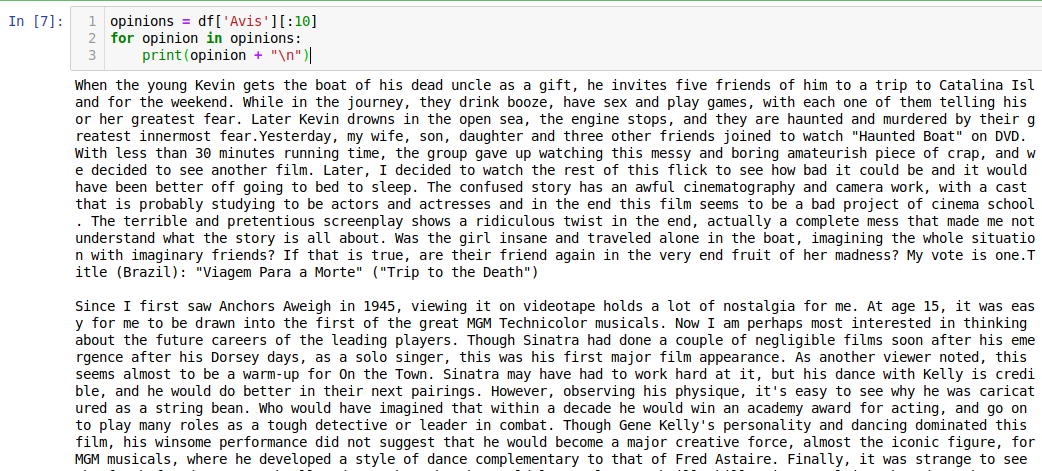
\includegraphics[scale=0.4]{images/snapshots/documents_sample.png}
  \caption{échantillon de documents}
  \label{fig:document_sample}
\end{figure}

\begin{figure}[!ht]
  \centering
  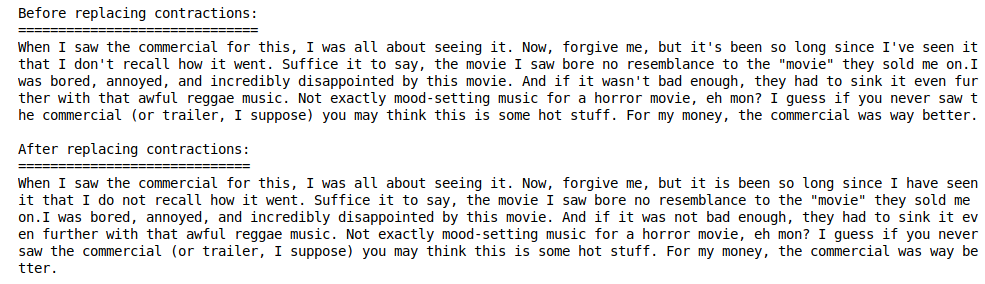
\includegraphics[scale=0.4]{images/snapshots/replace_contractions.png}
  \caption{remplacement des expressions contractées dans un document}
  \label{fig:replace_contractions}
\end{figure}

\begin{figure}[!ht]
  \centering
  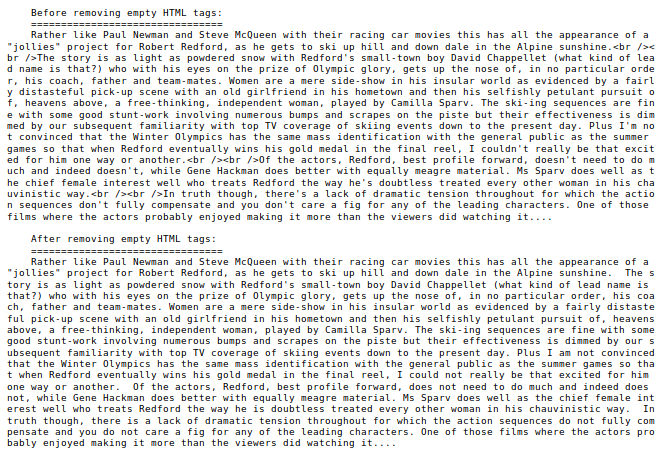
\includegraphics[scale=0.6]{images/snapshots/remove_empty_html_tags.png}
  \caption{suppression des balises auto-fermantes d'un document}
  \label{fig:remove_empty_html_tags}
\end{figure}

\begin{figure}[!ht]
  \centering
  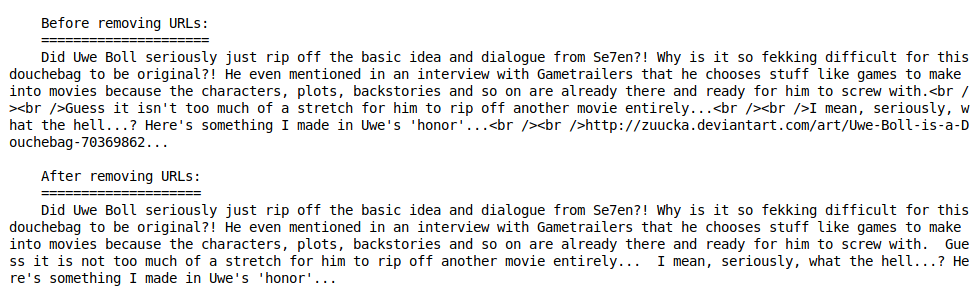
\includegraphics[scale=0.45]{images/snapshots/remove_urls.png}
  \caption{suppression des URLs d'un document}
  \label{fig:remove_urls}
\end{figure}

\begin{figure}[!ht]
  \centering
  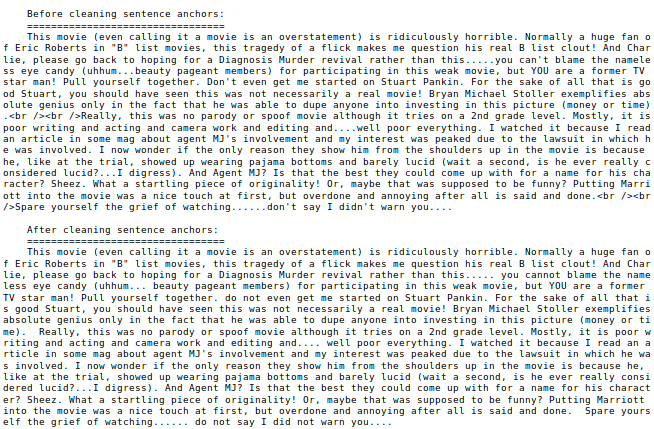
\includegraphics[scale=0.6]{images/snapshots/clean_sentence_anchors.png}
  \caption{nettoyage syntaxique des phrases mal commencées/terminées d'un document}
  \label{fig:clean_sentence_anchors}
\end{figure}

\begin{figure}[!ht]
  \centering
  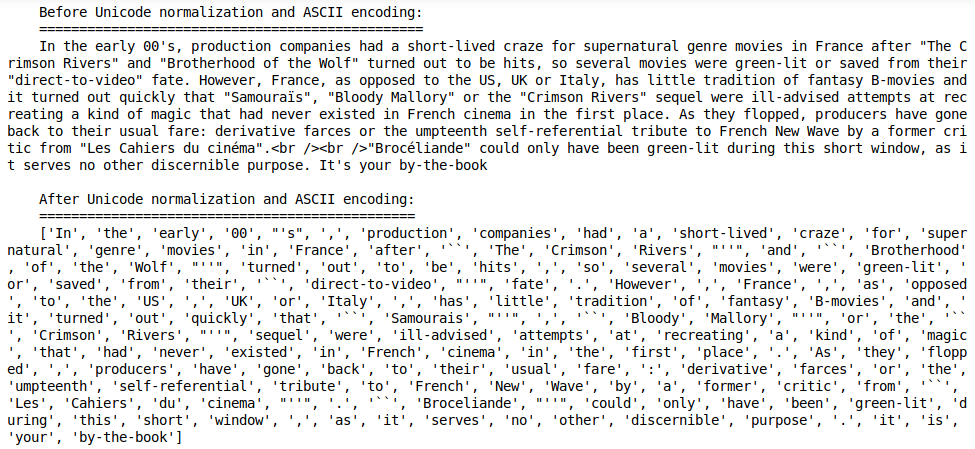
\includegraphics[scale=0.45]{images/snapshots/remove_non_ascii.png}
  \caption{normalisation Unicode, et encodage ASCII des tokens d'un document}
  \label{fig:remove_non_ascii}
\end{figure}

\begin{figure}[!ht]
  \centering
  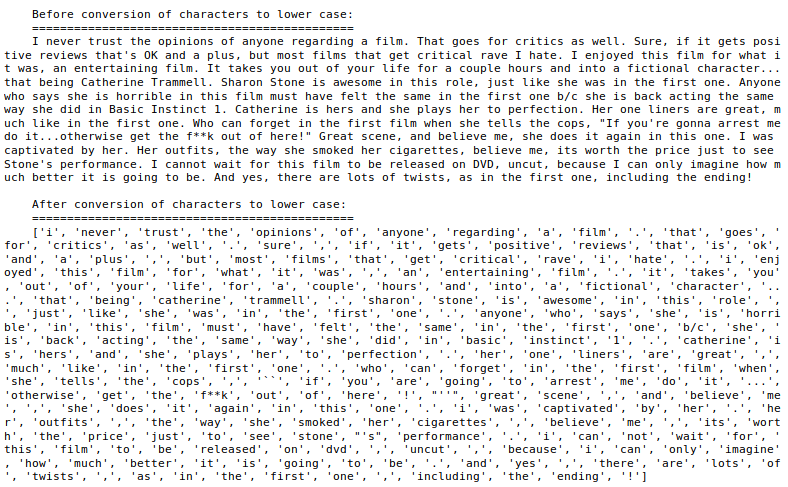
\includegraphics[scale=0.6]{images/snapshots/lowercase.png}
  \caption{conversion en minuscule des tokens d'un document}
  \label{fig:lowercase}
\end{figure}

\begin{figure}[!ht]
  \centering
  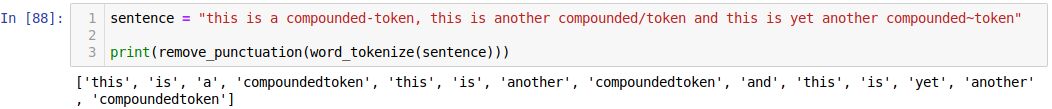
\includegraphics[scale=0.45]{images/snapshots/before_split_characterset.png}
  \caption{suppression des caractères de ponctuation, avant le découpage de tokens composés}
  \label{fig:before_split_characterset}
\end{figure}

\begin{figure}[!ht]
  \centering
  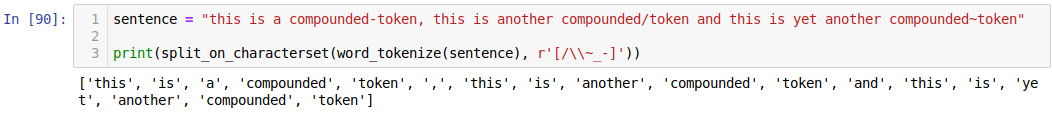
\includegraphics[scale=0.45]{images/snapshots/after_split_characterset.png}
  \caption{découpage des tokens composés}
  \label{fig:after_split_characterset}
\end{figure}

\begin{figure}[!ht]
  \centering
  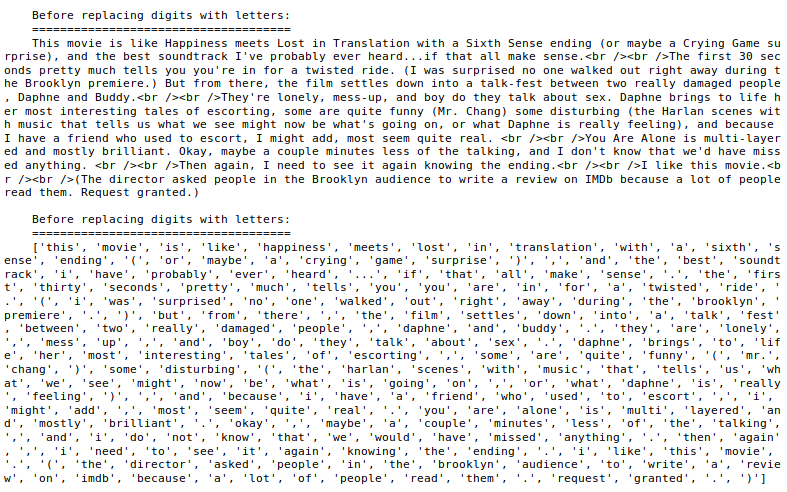
\includegraphics[scale=0.5]{images/snapshots/replace_numbers.png}
  \caption{remplacement des tokens désignant des chiffres par leurs équivalents en lettres}
  \label{fig:replace_numbers}
\end{figure}

\begin{figure}[!ht]
  \centering
  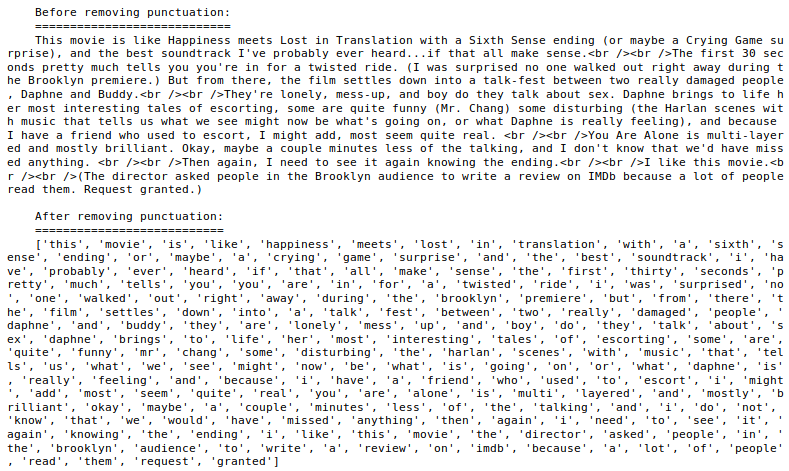
\includegraphics[scale=0.5]{images/snapshots/remove_punctuation.png}
  \caption{suppression des caractères de ponctuation}
  \label{fig:remove_punctuation}
\end{figure}

\begin{figure}[!ht]
  \centering
  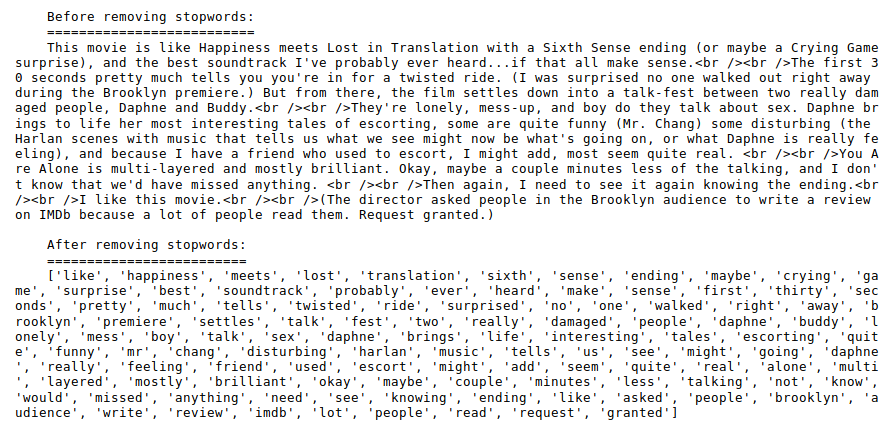
\includegraphics[scale=0.4]{images/snapshots/remove_stopwords.png}
  \caption{suppression des stopwords}
  \label{fig:remove_stopwords}
\end{figure}

\begin{figure}[!ht]
  \centering
  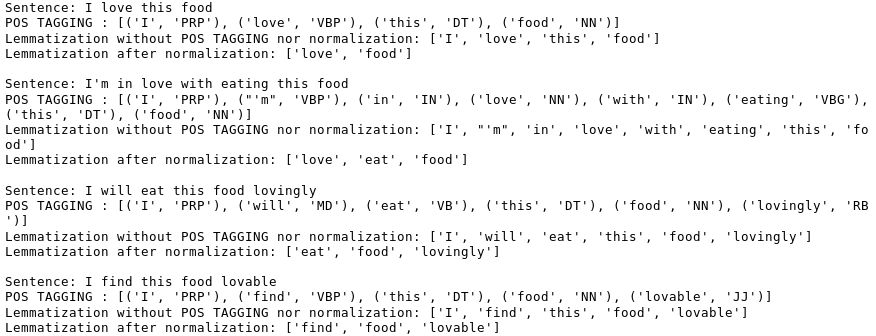
\includegraphics[scale=0.4]{images/snapshots/lemmatization.png}
  \caption{lemmatization en utilisant le POS-Tagging}
  \label{fig:lemmatization}
\end{figure}

\end{appendices}

\end{document}
